\documentclass{article}
\usepackage{times}
\usepackage{graphicx}
\usepackage{subfigure} 
\usepackage{natbib}
\usepackage{algorithm}
\usepackage[nice]{nicefrac}
\usepackage{algorithmic}
\usepackage{hyperref}
\newcommand{\theHalgorithm}{\arabic{algorithm}}
\usepackage{icml2017}
%\usepackage[accepted]{icml2017}

\def\bsa{{\boldsymbol\alpha}}
\def\bse{{\boldsymbol\epsilon}}
\def\bsk{{\boldsymbol\kappa}}
\def\bsm{{\boldsymbol\mu}}
\def\bsl{{\boldsymbol\lambda}}
\def\bsph{{\boldsymbol\phi}}
\def\bsth{{\boldsymbol\theta}}
\usepackage{amsmath}
\usepackage{amssymb}
\usepackage{amsfonts}
\usepackage{enumerate}
\usepackage{fullpage}
\usepackage{bbm}
\usepackage{caption}
\usepackage{mathrsfs}

\newcommand{\pa}[1]{ \left({#1}\right) }

\def \N {\mathbb{N}}
\def \Nbr {\mathcal{N}}
\def \mcL {\mathcal{L}}
\def \Q {\mathbb{Q}}
\def \F {\mathbb{F}}
\def \then {\implies &}
\def \oif {\Longleftrightarrow &\,}
\def \given {\text{Given }&}
\def \assume {\text{Assume }&}
\def \thfr {\therefore &\enskip}
\def \bij {\leftrightarrow}
\def \inj {\rightarrowtail}
\def \sur {\twoheadedrightarrow}
\def \Z {\mathbb{Z}}
\def \R {\mathbb{R}}
\def \C {\mathbb{C}}
\def \T {\mathbb{T}}
\def \iff {\Longleftrightarrow}
\def \kron {\boldsymbol\delta}
\def \indicator {\mathbbm{1}}

\def\Tx{\textbf{x}}
\def\TX{\textbf{X}}
\def\TU{\textbf{U}}
\def\Ty{\textbf{y}}
\def\tbr{\textbf{r}}
\def\Tz{\textbf{z}}
\def\quotient{\mathclose{}/\mathopen{}}
\def\Tf{\textbf{f}}
\def\Th{\textbf{h}}
\def\Tg{\textbf{g}}
\def\sumn{\sum_{n=0}^\infty}
\def\limn{\lim_{n\rightarrow\infty}}
\def\prodn{\prod_{n=0}^\infty}

\DeclareMathOperator\adj{adj}
\DeclareMathOperator\cov{cov}
\DeclareMathOperator\Unif{Unif}
\DeclareMathOperator\blockdiag{blockdiag}
\DeclareMathOperator\Pois{Pois}
\DeclareMathOperator\mathProb{\mathbb{P}}
\def\P{\mathProb} % need to overwrite stupid paragraph symbol
\DeclareMathOperator\mathExp{\mathbb{E}}
\def \E {\mathExp}


\newcommand{\stc}[1]{\widetilde{#1}}   
\newcommand{\set}[2]{ \left\{ #1 \,\middle|\, #2 \right\} }
\newcommand{\shift}[1]{&\quad & \text{#1}\\}
\newcommand{\lem}[1]{\text{\textbf{L.\ref{#1}}}}
\newcommand{\card}[1]{\left\vert{#1}\right\vert}
\newcommand{\Ps}[1]{\mathcal{P}\left({ #1 }\right)}
\newcommand{\colv}[1]{\begin{pmatrix} #1 \end{pmatrix}}
\newcommand{\mat}[1]{\begin{pmatrix} #1 \end{pmatrix}}
\newcommand{\detmat}[1]{\begin{vmatrix} #1 \end{vmatrix}}
\newcommand{\spanb}[1]{\text{span}\{ #1 \}}
\newcommand{\abs}[1]{\left|#1\right|}
\newcommand{\Inner}[1]{\langle #1 \rangle}
\newcommand{\Innercpy}[1]{\langle #1, #1 \rangle}
\newcommand{\norm}[1]{\mathopen\| #1 \mathclose\|}% use instead of $\|x\|$

\def\eqd{\mathrel{\overset{\Delta}{=}}}

\DeclareMathOperator{\diag}{diag}
\DeclareMathOperator{\vcdim}{VC-dim}
\DeclareMathOperator*{\Err}{\text{err}}
\DeclareMathOperator*{\ErrE}{\mathbb{E}}
\DeclareMathOperator{\Tr}{tr}
\DeclareMathOperator{\Dim}{dim}
\DeclareMathOperator{\Rank}{rank}
\DeclareMathOperator*{\argmin}{argmin}
\DeclareMathOperator*{\proj}{proj}
\DeclareMathOperator{\Ker}{ker}
\DeclareMathOperator{\Diam}{diam}
\DeclareMathOperator{\Int}{int}
\DeclareMathOperator{\Clo}{clo}
\DeclareMathOperator{\sgn}{sgn}
\DeclareMathOperator{\MyRe}{Re}
\DeclareMathOperator{\MyIm}{Im}
\DeclareMathOperator{\Supp}{supp}
\DeclareMathOperator{\Var}{Var}

% probability stuff
\def \sa {{$\sigma$-algebra}}
\def\OR{{\overline{\R}}}
\def\OX{{\overline{X}}}


\def \mcX {\mathcal{X}}
\def \mcY {\mathcal{Y}}
\def \mcH {\mathcal{H}}
\def \mcD {\mathcal{D}}
\def \mcA {\mathcal{A}}
\def \mcK {\mathcal{K}}
\def\mcG{{\mathcal{G}}}
\def\mcH{{\mathcal{H}}}
\def\mcF{{\mathcal{F}}}
\def\mcB{{\mathcal{B}}}
\def\mcE{{\mathcal{E}}}
\def\mcP{{\mathcal{P}}}
\def\mcM{{\mathcal{M}}}
\def\mcC{{\mathcal{C}}}
\def\mcT{{\mathcal{T}}}

% \icmltitlerunning{Submission and Formatting Instructions for ICML 2017}

\begin{document} 

\twocolumn[
\icmltitle{Large Linear Multi-output Gaussian Process Learning}
%\icmlsetsymbol{equal}{*}
\begin{icmlauthorlist}
  \icmlauthor{Vladimir Feinberg}{pu}
  \icmlauthor{Li-Fang Cheng}{pu}
  \icmlauthor{Barbara E. Engelhardt}{pu}
  \icmlauthor{Kai Li}{pu}
\end{icmlauthorlist}
\icmlaffiliation{pu}{Princeton University, Princeton, USA}
\icmlcorrespondingauthor{Vladimir Feinberg}{vyf@princeton.edu}

\icmlkeywords{multi-task, multi-output, Gaussian process, large scale}

\vskip 0.3in
]
\printAffiliationsAndNotice{}
%\printAffiliationsAndNotice{\icmlEqualContribution}

\begin{abstract}
Gaussian process (GP) models, which put a distribution over arbitrary functions in a continuous domain, can be generalized to the multi-output case; a common way of doing this is to use a linear model of coregionalization \cite{alvarez2012kernels}. Such models can learn correlations across the multiple outputs, such as temperature data from disparate regions, which can then be exploited to share knowledge across the multiple outputs. While model learning can be performed efficiently for single-output GPs, the multi-output case still requires approximations for large $n$, the total number of observations across all outputs. In this work, we describe a new method, Large Linear GP (LLGP), which estimates covariance hyperparameters for multi-dimensional outputs and one-dimensional inputs. We show results of our approach applied to real time series data, and compare these results against related methods. Finally, we explore extensions of our approach to multidimensional inputs.
\end{abstract} 

\section{Introduction}
\label{introduction}

Gaussian processes (GPs) are a popular nonlinear regression method that innately capture function smoothness across inputs as defined by their covariance function \cite{williams1996gaussian}. GPs seamlessly extend to multi-output learning, picking up on latent cross-output processes, where in multi-output learning the objective is to build a probabilistic regression model over vector-valued observations.

Such an extension is especially important in time series data, where multi-output GPs have been applied to the problem of imputing missing temperature readings for sensors in different locations and reconstructing missing foreign exchange rates and commodity prices given rates and prices for other goods over time \cite{osborne2008towards, alvarez2010efficient}.

Exact GP inference comes at a cost: to compute the gradients for kernel hyperparameters, an exact computation requires an $O(n^3)$ decomposition of an $O(n^2)$ matrix in memory for $n$ samples \cite{gpml}. Each hyperparameter's scalar partial derivative then requires another $O(n^2)$ computation. While these operations may be performed in parallel, the memory use and runtime is prohibitive for problems with a large number of outputs, since the number of hyperparameters grows accordingly. For this reason, an accurate approximate approach has been an important goal of machine learning research.

For a single output, variational approaches that work on $m\ll n$ inducing points, or locations at which the true kernel is sampled, letting users trade off accuracy for efficiency \cite{hensman2013gaussian}.

Nguyen and Bonilla observed in Collaborative Multi-output Gaussian Processes (COGP) that multi-output GP algorithms can further share an internal representation of the covariance structure among all outputs at once \yrcite{nguyen2014collaborative}. We analogously exploit sharing in the covariance structure.

\subsection{Contributions}

Our approach makes the following contributions to approximate inference in multi-output GPs. First, we identify a block-Toeplitz structure induced by the linear model of coregionalization (LMC) kernel on a grid. Next, we adapt a previously identified kernel structure based on Semiparametric Latent Factor Models (SLFM) \cite{seeger2005semiparametric}. Both of these structures coordinate for fast matrix-vector multiplication $K\Ty$ with the covariance matrix $K$.

When inputs do not lie on a uniform grid (i.e., for time series, the length of time between observations differs), we apply a technique proposed in Massively Scalable Gaussian Processes (MSGP) \cite{msgp}. For single-output kernels, MSGP leverages the structured kernel interpolation (SKI) framework to make inputs act as if they are on a grid \cite{kiss-gp}. In a single-output case, this opens up the possibility for a matrix-free GP, avoiding construction of the explicit Gram covariance matrix. Because LMC kernels exhibit the previously-identified block-Toeplitz structure, they harmonize with SKI. While direct application of SKI is not possible, we can make an extension that makes matrix-free LMC kernel learning viable even on non-grid inputs.

Our paper is organized as follows. In Section~\ref{sec:background} we give a background on single-output and multi-output GPs, as well as some history in structured linear algebra in GPs. Section~\ref{sec:related-work} details both related work that was built upon in LLGP and existing methods for multi-output GPs. Section~\ref{sec:matrix-free} describes our method, including a matrix-free heuristic stopping criterion. Then, in Section~\ref{sec:results} we compare the performance of LLGP to existing methods and offer concluding remarks in Section~\ref{conclusion}.

\section{Background}
\label{sec:background}
\subsection{General Gaussian processes}

First, we give an overview of the theoretical foundation for GPs. A GP is a set of random variables (RVs) $\{f_\Tx\}_\Tx$ indexed by $\Tx\in\mcX$, with the property that for any finite collection $X\subset\mcX$, the RVs are jointly Gaussian with a prescribed mean function $\bsm:\mcX\rightarrow\R$ and covariance $K:\mcX^2\rightarrow\R$, i.e., $f_X\sim N\pa{\bsm_X, K_{X, X}}$ \cite{williams1996gaussian}. As usual, we drop the mean with $\Ty\triangleq f_X-\bsm_X$ and denote vectorization $f_X=\colv{f_{\Tx}}_{\Tx\in X}$ or matricization $K_{X,Z}=\mat{K(\Tx,\Tz)}_{\Tx\in X,\Tz\in Z}$ with subscripts.

Given a set of $n$ observations at each $X$ of the $\R^n$-valued RV $\Ty$, inference at a single point $*\in\mcX$ of an $\R$-valued RV $y_*$ is performed by marginalization \cite{gpml}:
\begin{equation*}
y_*|\Ty\sim N\pa{K_{*, {X}}K^{-1}_{{X}, {X}}\Ty, K_{*, *}-K_{*, {X}}K^{-1}_{{X}, {X}}K_{{X}, *}}.
\end{equation*}
Accuracy is often sensitive to a particular parameterization of our kernel, so model estimation is performed by maximizing data log likelihood with respect to parameters $\bsth$ of $K$:
\begin{align}
  \mcL(\bsth)&=\log p(\Tf_{X}|X,\bsth)\label{datall}\\
             &=-\frac{1}{2}\Ty^\top K_{|\bsth}^{-1}\Ty-\frac{1}{2}\log \abs{K_{|\bsth}}-\frac{n}{2}\log 2\pi.\nonumber
\end{align}
As such, the heart of GP learning lies in optimization of $\mcL$. Gradient-based optimization methods then require the gradient with respect to every parameter $\theta_j$ using $\bsa=K_{|\bsth}^{-1}\Ty$:
\begin{align}
\partial_{\theta_j}\mcL = \frac{1}{2}\bsa^\top\partial_{\theta_j}K_{|\bsth}\bsa -\frac{1}{2}\Tr\pa{K_{|\bsth}^{-1}\partial_{\theta_j}K_{|\bsth}}.\label{llgradient}
\end{align}

\subsection{Multi-output linear GPs}

We build multi-output GP models as instances of general GPs, where a multi-output GP model identifies correlations between outputs through a shared input space \cite{alvarez2012kernels}.

Here, for $D$ outputs, we write our indexing set as $\mcX'=[D]\times \mcX$: an input is in a point from a shared domain coupled with an output tag. Then, if we make observations at $X_d\subset\mcX$ for output $d\in[D]$, we can set:
\begin{align*}
\TX=\set{(d, x)}{d\in[D],x\in X_d}\subset{\mcX'};\;\; n=\card{\TX}.
\end{align*}

An LMC kernel $K$ is of the form 
\begin{align}
K([i,\Tx_i],[j,\Tx_j])=\sum_{q=1}^Qb_{ij}^{(q)}k_q(\norm{\Tx_i-\Tx_j})+\epsilon_i\delta_{ij},\label{lmcpointwise}
\end{align} 
where $k_q:\R\rightarrow\R$ is a stationary kernel on $\mcX$. Typically, the positive semi-definite (PSD) matrices $B_q\in\R^{D\times D}$ formed by $b_{ij}^{(q)}$ are parameterized as $A_qA_q^\top+\bsk_q I_D$, with $A_q\in\R^{D\times R_q},\bsk_q\in\R_+^D$ and $R_q$ a preset rank. Importantly, even though each $k_q$ is stationary, $K$ is only stationary on $\mcX'$ if $B_q$ is Toeplitz. Settings of $B_q$ that arise in practice, where we wish to capture covariance across outputs as an arbitrary $D^2$-dimensional latent process,  prevent stationarity in $K$ and therefore prohibit direct application of SKI.

\subsection{Structured covariance matrices}

If we can identify structure in the covariance matrices $K$, then we can recover fast in-memory representations and efficient matrix-vector multiplications (MVMs) for $K$.

The Kronecker product $A\otimes B$ of matrices of order $a,b$ is a block matrix of order $ab$ with $ij$-th block $A_{ij}B$. We can represent it by keeping representations of $A$ and $B$ separately, rather than the product. Then, the corresponding MVMs can be computed in time $O(a\text{MVM}(B)+b\text{MVM}(A))$, where $\text{MVM}(\cdot)$ is the runtime of a MVM. For GPs on uniform dimension-$P$ grids, this approximately reduces the runtime and representation costs by a $(1/P)$-th power \cite{gilboa2015scaling}.

Symmetric Toeplitz matrices $T$ are constant along their diagonal and fully determined by their top row $\{T_{1j}\}_j$, yielding an $O(n)$ representation. Such matrices arise naturally when we examine the covariance matrix induced by a stationary kernel $k$ applied to a one-dimensional grid of inputs. Since the difference in adjacent inputs $t_{i+1}-t_{i}$ is the same for all $i$, we have the Toeplitz property that:
\[
T_{(i+1)(j+1)}=k(\abs{t_{i+1} -t_{j+1}})=k(\abs{t_i-t_j})=T_{ij}
\]
Furthermore, we can embed $T$ in the upper-left corner of a circulant matrix $C$ of twice its size, which enables MVMs  $C\mat{\Tx\\\textbf{0}}=\mat{T\Tx\\\textbf{0}}$ in $O(n\log n)$ time. This approach has been used for fast inference in single-output GP time series with uniformly spaced inputs \cite{cunningham2008fast}.

\section{Related Work}
\label{sec:related-work}
\subsection{Approximate inference methods}

To cope with the lack of tractable GP inference methods, inducing point approaches create a tractable model to use instead of the classic GP. Such approaches fix or estimate inducing points $\TU$ and claim that the data $f_X$ is conditionally deterministic (deterministic training conditional, or DTC), independent (fully independent training conditional, or FITC), or partially independent (partially independent training conditional, or PITC) given RVs $f_{\TU}$  \cite{quinonero2005unifying}. These approaches are agnostic to kernel stationarity, and their quality can be improved by increasing the number of inducing points at the cost of a longer runtime. Setting the inducing points $\TU=\TX$ recovers the original exact GP.

In the context of LMC, a framework for variational DTC, DTCVAR, provided a matrix-free method where each iteration has complexity $O(n(Dm)^2)$, where $m$ is the average number of inducing points per output, $\card{\TU}/D$ \cite{alvarez2010efficient}. 

By sharing the $m$ inducing points across all outputs, Collaborative Multi-output Gaussian Processes (COGP) improves runtime per iteration to $O(m^3)$. Moreover, COGP only requires $O(Dnm)$ memory \cite{nguyen2014collaborative}. To ensure that $O(m^3)$ is computationally tractable for COGP, $m$ must be sufficiently small. COGP makes large multi-output GP estimation feasible through a variational approximation, the evidence lower bound, to the log likelihood.

\subsection{Approaches for stationary kernels}

\subsubsection{Structured Kernel Interpolation (SKI)}\label{ski-section}

SKI abandons the inducing-point approach: instead of using an intrinsically sparse model, SKI approximates the original $K_{X,X}$ directly \cite{kiss-gp}. To do this efficiently, SKI relies on the differentiability of $K$. For $\Tx,\Tz$ within a grid $U$, $\card{U}=m$, and $W_{\Tx,U}\in\R^{1\times m}$ as the cubic interpolation weights~\cite{keys1981cubic}, $\abs{K_{\Tx,\Tz}-W_{\Tx,U}K_{U,\Tz}}=O(m^{-3})$. The simultaneous interpolation $W\triangleq W_{X,U}\in\R^{n\times m}$ then yields the SKI approximation: $K_{X,X}\approx WK_{U,U}W^\top$. Importantly, $W$ has only $4^dn$ nonzero entries, with $\mcX=\R^d$.

In order to adapt SKI to our context of multiple outputs, we build grid $\TU\subset\mcX'$ out of a common subgrid $U\subset\mcX$ that extends to all outputs with $\TU = [D]\times U$. Since the LMC kernel evaluated between two sets of outputs $K_{X_i,X_j}$ is differentiable, as long as $U$ contains each $\{X_d\}_{d\in[D]}$, the corresponding SKI approximation $K_{\TX,\TX}\approx WK_{\TU,\TU}W^\top$ holds with the same asymptotic convergence cubic in $1/m$.

Massively Scalable Gaussian Processes (MSGP) observes that the kernel $K_{U,U}$ on a grid exhibits Kronecker and Toeplitz matrix structure \cite{msgp}. Drawing on previous work on structured GPs \cite{cunningham2008fast, gilboa2015scaling}, MSGP uses linear conjugate gradient descent as a method for evaluating $K_{|\bsth}^{-1}\Ty$ efficiently for Eq.~\ref{datall}. In addition, \cite{wilson2014fast} mentions an efficient eigendecomposition that carries over to the SKI kernel for the remaining $\log\abs{K_{|\bsth}}$ term in Eq.~\ref{datall}.

While evaluating $\log\abs{K_{|\bsth}}$ is not feasible in the LMC setting (because the LMC sum breaks Kronecker and Toeplitz structure), the general notion of creating structure with SKI carries over to LLGP.

\section{Matrix-free LMC Learning} \label{sec:matrix-free}

We propose a linear model of coregionalization (LMC) method based on recent structure-based optimizations for GP estimation instead of variational approaches. Critically, the accuracy of the method need not be reduced by keeping $m$ low because its reliance on structure allows better asymptotic performance.
For simplicity, our work focuses on multi-dimensional outputs, one-dimensional inputs, and Gaussian likelihoods.

\subsection{Matrix-free GP Learning}

Gibbs and MacKay describe the algorithm for GP model learning in terms of only MVMs with the covariance matrix \yrcite{gibbs1996cient}. In particular, they note that we can solve for $\bsa$ satisfying $K_{|\bsth}\bsa=\Ty$ in Eq.~\ref{llgradient} using linear conjugate gradient descent (LCG). Moreover, they develop a stochastic approximation by introducing RV $\tbr$ with $\cov \tbr=I$:
\begin{align}
  \Tr\pa{K_{|\bsth}^{-1}\partial_{\theta_j}K_{|\bsth}} = \E\left[(K_{|\bsth}^{-1}\tbr)^\top\partial_{\theta_j}K_{|\bsth}\tbr\right]\label{eq:trace}
\end{align}
For this approximation, the number of samples need not be large, and the estimate improves as the size of $K_{|\bsth}$ increases.
As in other work \cite{cutajar2016preconditioning}, we let $\tbr\sim\Unif\{\pm 1\}$.

We depart from Gibbs and MacKay in selecting MINRES instead of LCG as the Krylov-subspace inversion method used to compute inverses from MVMs. MINRES handles numerically semidefinite matrices with more grace \cite{fong2012cg}. This is essential in GP optimization, where the diagonal noise matrix $\bse$, iid for each output, shrinks over the course of learning, making inversion-based methods require additional iterations (Fig.~\ref{fx2007-iterations}).

\begin{figure}[!ht]
\vskip 0.1in
\begin{center}
\centerline{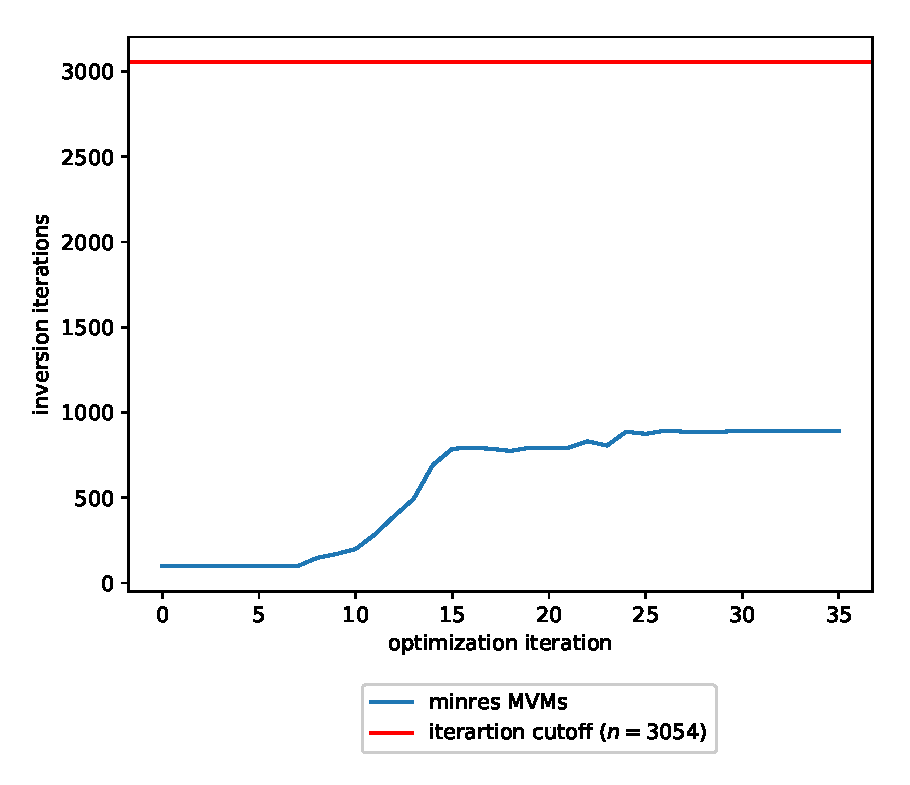
\includegraphics[width=\columnwidth]{iterations.eps}}
\caption{Number of MVMs that MINRES must perform at each optimization iteration for a GP applied to the dataset in Section~\ref{fx2007-results}. The iteration cutoff is the number of training points $n$ in the dataset.
}
\label{fx2007-iterations}
\end{center}
\vskip -0.1in
\end{figure}

If we sample $N_t$ instances of $\tbr$, every iteration needs to perform $N_t+1$ inversions including $\Ty$, if we reuse the same samples $K_{|\bsth}^{-1}\tbr$ between derivatives $\partial_{\theta_j}$. These inversions are done in parallel. Then, since $\partial_{\theta_j}K_{|\bsth}$ is both structured and smaller than $K_{|\bsth}$, each of the terms in the approximation Eq.~\ref{eq:trace} require $\tilde{O}(n)$ time to compute.

Critically, we cannot access $\mcL$ itself, only $\nabla\mcL$, so we choose AdaDelta as the high-level optimization routine \cite{zeiler2012adadelta}. We considered several stochastic approximations for finding $\log\abs{K_{|\bsth}}$~\cite{dorn2015stochastic, han2015large}, but found these too slow and inaccurate for use in optimization.

In other words, all the work is done in the inversions $K_{|\bsth}^{-1}\tbr,K_{|\bsth}^{-1}\Ty$, which in turn rely on the MVM operation, discussed in Section~\ref{fast-mvm}. Since $K_{|\bsth}$ only enters computation as an MVM operator, the amount of memory consumed is dictated by its representation, which need not be dense.

\subsection{Fast MVMs and parsimonious kernels}\label{fast-mvm}

When LMC kernels are evaluated on a grid of points for each output, so $X_d=U$, the simultaneous covariance matrix equation without noise Eq.~\ref{lmcgrid} over $\TU$ holds for Toeplitz matrices $K_q$ formed by the stationary kernels $k_q$ evaluated at pairs of $U\times U$.
\begin{align}
  K_{\TU,\TU}=\sum_q(A_qA_q^\top+\diag\bsk_q)\otimes K_q\label{lmcgrid}
\end{align}
The SLFM and COGP models correspond to all $\bsk_q$ set to 0 and $A_q=\textbf{a}_q\in\R^{D\times 1}$. Moreover, we include $D$ additional kernels for the independent GP components, which can be incorporated using kernels $K_d$ where $A_d=0$ and $\bsk_d$ as the $d$th standard basis vector of $\R^D$ for $d\in[D]$. This shows a reduction from SLFM to LMC.

Importantly, the Kronecker structure of Eq.~\ref{lmcgrid} lets us re-use the same grid $K_q$ in a computational sense across the different outputs. Recalling our SKI extension to multiple outputs (Section~\ref{ski-section}), we build a corresponding approximation for the differentiable part of our kernel:
\begin{align}
  K_{\TX,\TX}\approx WK_{\TU,\TU}W^\top+\bse.\label{lmcski}
\end{align}
We cannot fold $\bse$ into the interpolated term $K_{\TU,\TU}$ since it does not correspond to a differentiable kernel, so the SKI approximation fails. But this fact does not prevent efficient representation or multiplication since the matrix is diagonal. In particular, the MVM operation $K_{\TX,\TX}\Tx$ can be approximated by $WK_{\TU,\TU}W^\top\Tx+\bse\Tx$, where matrix multiplication by the sparse matrices $\bse, W,W^\top$ require $O(n)$ space and time.

We consider different representations of $K_{\TU,\TU}$ from (Eq.~\ref{lmcski}) to reduce the memory and runtime overhead for performing the multiplication $K_{\TU,\TU}\Tz$ (where we have computed $\Tz=W^\top\Tx$).

\subsubsection{\textsc{sum}: sum representation}

In \textsc{sum}, we represent $K_{\TU,\TU}$ with a $Q$-length list. At each index $q$, $B_q$ is a dense matrix of order $D$ and $K_q$ is a Toeplitz matrix of order $m$, where only its top row needs to be represented to perform MVMs.

In turn, multiplication $K_{\TU,\TU}\Tz$ is performed by multiplying each matrix in the list with $\Tz$ and summing the results, corresponding to . As described before, the Kronecker MVM $(B_q\otimes K_q)\Tz$ may be expressed as $D$ fast Toeplitz MVMs with $K_q$ and $m$ dense MVMs with $B_q$. In turn, the runtime for each of the $Q$ terms is $O(Dm\log m)$.

\subsubsection{\textsc{bt}: block-Toeplitz representation}

In \textsc{bt}, we notice that $K_{\TU,\TU}$ is a block matrix with blocks $T_{ij}$:
\begin{align*}
\sum_qB_q\otimes K_q =\mat{T_{ij}}_{i,j\in[D]^2},\;\; T_{ij}=\sum_qb_{ij}^{(q)}K_q.
\end{align*}
On a one-dimensional grid $U$, these matrices are Toeplitz since they are linear combinations of Toeplitz matrices. \textsc{bt} requires $D^2$ $m$-sized rows to represent each $T_{ij}$. Then, using usual block matrix multiplication, an MVM $K_{\TU,\TU}\Tz$ takes $O(D^2m\log m)$ time.

\subsubsection{\textsc{slfm}: SLFM representation}

\textsc{slfm} uses a rank-based representation. Let $R\triangleq \nicefrac{\sum_qR_q}{Q}$ be the average added rank, $R\le D$.

We first rewrite the grid kernel:
\begin{align*}
  K_{U,U}=\sum_q\sum_{r=1}^{R_q}\textbf{a}_q^{(r)}{\textbf{a}_q^{(r)}}^\top\otimes K_q + \sum_q\diag\bsk_q \otimes K_q.
\end{align*}
Note $\textbf{a}_q^{(r)}{\textbf{a}_q^{(r)}}^\top$ is rank-1. Under some re-indexing $q'\in[RQ]$ which flattens the double sum such that each $q'$ corresponds to a unique $(r, q)$, the term $\sum_q\sum_{r=1}^{R_q}\textbf{a}_q^{(r)}{\textbf{a}_q^{(r)}}^\top\otimes K_q $ may be rewritten as
\begin{align*}
  \sum_{q'}\textbf{a}_{q'}\textbf{a}_{q'}^\top\otimes K_{q'} = \textbf{A}\blockdiag_{q'}\colv{K_{q'}}\textbf{A}^\top;
\end{align*}
where the second simplification has $\textbf{A}=\mat{ \textbf{a}_{q'}}_{q'}\otimes I_m$ with $\mat{ \textbf{a}_{q'}}_{q'}$ a matrix of horizontally stacked column vectors \cite{seeger2005semiparametric}. Next, we rearrange the remaining term $\sum_q\diag\bsk_q \otimes K_q$ as $\blockdiag_d(T_d)$, where $T_d=\sum_q \kappa_{qd}K_q$ is Toeplitz.

Thus, the \textsc{slfm} representation writes $K_{\TU,\TU}$ as the sum of two block diagonal matrices of block order $QR$ and $D$, where each block is a Toeplitz order $m$ matrix, so MVMs take $O((QR + D)m\log m)$ time.

\subsection{Asymptotic performance}

Because the runtimes of \textsc{bt} and \textsc{slfm} are complimentary in the sense that one performs better than the other when $D^2>QR$ and vice-versa, an algorithm that uses the aforementioned condition between to decide between which representation to use can minimize runtime. We also found that \textsc{sum} is efficient in practice for $Q=1$.

Using the switching condition, MVMs with the original matrix $K_{\TX,\TX}$ altogether have a space and time upper bound of $\tilde{O}(\min(QR,D^2)m+n)$, where the $\min$ is earned thanks to the choice between different representations. Every AdaDelta iteration then takes $\tilde{O}(\sqrt{\kappa_2})$ such matrix-vector products for machine-precision answers, with $\kappa_2$ the spectral condition number \cite{raykar2007fast}.

On a grid of inputs with $\TX=\TU$, the SKI interpolation vanishes with $W=I$. In this case, using \textsc{bt} alone leads to a faster algorithm---applying the Chan block-Toeplitz preconditioner in a Krylov-subspace based routine has experimentally shown convergence using fewer MVMs \cite{chan1994circulant}.

\subsection{Stopping conditions}\label{stopping}

For a gradient-only stopping heuristic, we maintain the running maximum gradient $\infty$-norm. If gradient norms drop below a preset proportion of the running maximum norm more than a pre-set tolerance number of times, we terminate. For example, when applied to the foreign exchange rate prediction (FX2007) dataset in Section~\ref{fx2007-results}, the heuristic eventually notices that we have slowed down increases in $\mcL$ because the gradients occasionally drop below the threshold at that point, while not displacing the solution $\bsth$ significantly since we must be near a local minimum (Fig.~\ref{fx2007-stop}). 

\begin{figure}[!ht]
\vskip 0.1in
\begin{center}
\centerline{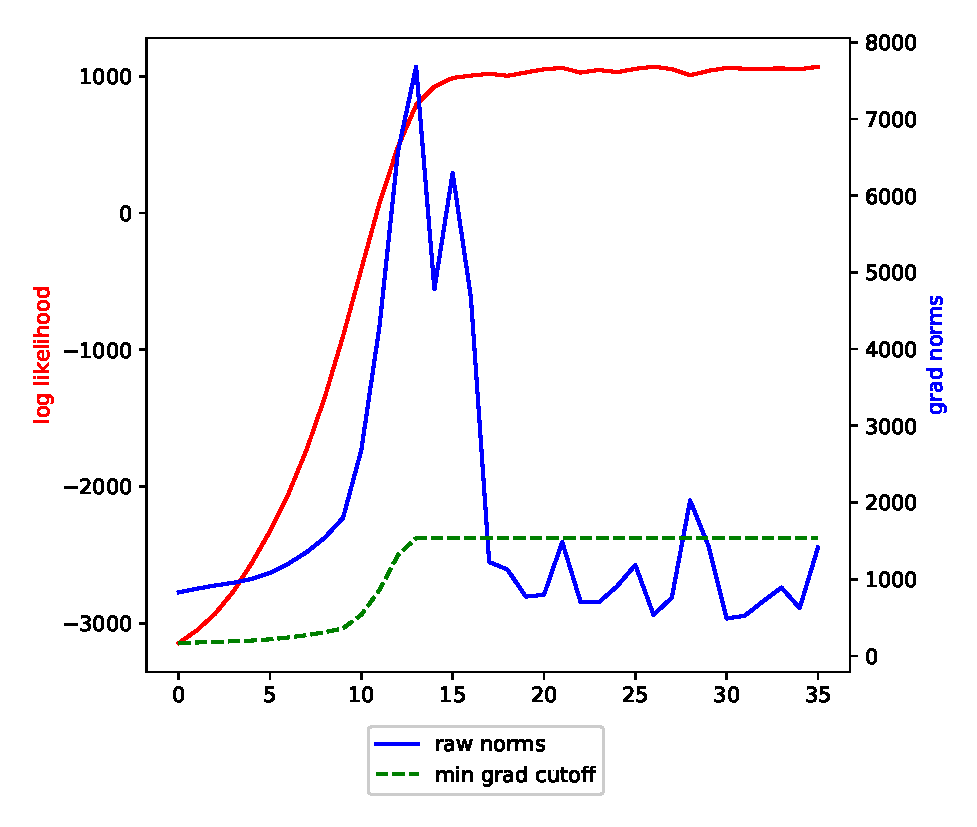
\includegraphics[width=\columnwidth]{running_cutoff.eps}}
\caption{In green, we have 20\% of the rolling maximum norm. In red and blue are $\mcL$ (computed exactly and therefore unavailable during benchmarks) and $ \norm{\nabla\mcL}_\infty $, respectively. }
\label{fx2007-stop}
\end{center}
\vskip -0.1in
\end{figure}

\subsection{Prediction}

The predictive mean can be computed in $O(1)$ time as observed in \cite{msgp} by $K_{*,X}\bsa\approx W_{*,\TU}K_{\TU,\TU}\bsa$.

The full predictive covariance estimate requires finding a new term $K_{*,X}K_{X,X}^{-1}K_{X,*}$. This is done by solving the linear system in a matrix-free manner on-the-fly; in particular, $K_{X,X}^{-1}K_{X,*}$ is computed via MINRES for every new test point $K_{X,*}$. Over several test points, this is embarrassingly parallelizable.

A more efficient predictive variance algorithm is outside the scope of this paper: for a research setting, we expect training time to be the bottleneck. Moreover, one can couple LLGP learning with other prediction mechanisms. One example is the sampling-based approach proposed in \cite{papandreou2011efficient}, which extends to linear combinations of kernels that allow fast eigendecompositions.

\subsection{Hyperparameter Settings}

AdaDelta parameters were set to the following on all tests: rate $=1$, decay $=0.9$, momentum $=0.5$, offset $=0.0001$. The stopping criterion parameters permit the gradient $\infty$-norm to drop below a threshold of its maximum value so far a small, fixed number of times, 5. The maximum number of iterations was 100.

For learning, we initialize entries $A_q$ according to a unit normal and all $\bsk_q$ to $1$. Note that COGP initializes the coregionalization matrix to $1$ uniformly. Like COGP, we initialize noise to $0.1$ for all outputs.

\section{Results}
\label{sec:results}
We evaluate the methods on held out data by using standardized mean square error (SMSE) of the test points with the predicted mean, and the negative log predictive density (NLPD) of the Gaussian likelihood of the inferred model. Notably, NLPD takes confidence into account, while SMSE only evaluates the mean prediction. In both cases, lower values represent better performance. 

\subsection{Representation evaluation}\label{empirical-rep}

We evaluated the performance of the different kernel representations over various rank and parameterization settings. In particular, we have the following parameters: $n$ total sample size across all outputs, $D$ number of outputs, $Q$ number of kernels $k_q$, $R$ average added rank, $\epsilon$ mean noise, and \texttt{ktype} kernel type. Kernel type is one of \texttt{mat, periodic, rbf, mix} corresponding to Mat\'{e}rn-3/2, standard periodic\footnote{We define the periodic kernel as $k(r) = \exp \left(\frac{-\gamma}{2}\sin^2\frac{\pi r}{T}\right)$.}, and radial basis functions. \texttt{mix} refers to a mix of all three kernels.

Each kernel's inverse length scales and periods were selected by sampling uniformly in log space from 1 to 10 with $Q$ samples. Next, we construct a random LMC kernel by sampling entries of each $A_q$ from a standard normal distribution, $\bsk_q$ from an inverse gamma with unit shape and scale, and independent noise $\bse$ for every output from an inverse gamma with unit scale and mean $\epsilon$. Inputs and outputs were independently generated from $\Unif[0,1]$ for benchmarking.

As expected from their asymptotic runtime, \textsc{sum}, \textsc{bt}, and \textsc{slfm} representations are complimentary in MVM speed for different configurations of $D,R,Q$---this results in sparse inversion computation that consistently outperforms Cholesky decomposition in runtime (Tab.~\ref{complement}).
For inverting systems, all computations were carried out until the residual $\ell_2$ norm was at most $10^{-4}$.
\begin{table}[!ht]
  \caption{The runtime in seconds for solving $K\Tx=\Ty$ for a random kernel $K$ constructed as in Section~\ref{empirical-rep} using MINRES for each of the kernel representations. For comparison, the \textsc{chol} representation is wallclock time to compute the Cholesky decomposition of the matrix, which must be constructed, and use this decomposition to invert the system. We averaged over five runs. In every run, we use $n=5000$ simulated data points, $\texttt{mix}$ kernels, and $\epsilon=0.1$.
}
\label{complement}
\vskip 0.15in
\begin{center}
  \begin{small}
    
\begin{tabular}{|ccc|cccc|}
  \hline
  \abovespace\belowspace
  $D$ & $R$ & $Q$ & \textsc{cholesky} & \textsc{sum} & \textsc{bt} & \textsc{slfm}\\
\hline
  \abovespace
 $ 2 $ & $ 2 $ & $ 10 $ & $ 41.00 $ & $ 32.24 $ & $ \textbf{6.53} $ & $ 42.33 $ \\ 
 $ 10 $ & $ 1 $ & $ 10 $ & $ 37.38 $ & $ 31.01 $ & $ 20.81 $ & $ \textbf{9.34} $ \\ 
 $ 10 $ & $ 10 $ & $ 1 $ & $ 10.74 $ & $ \textbf{0.41} $ & $ 2.40 $ & $ 0.89 $ 
  \belowspace \\

  \hline
\end{tabular}

\end{small}
\end{center}
\vskip -0.1in
\end{table}

We next evaluated the accuracy of the gradients for $N_t=10$ trace samples. Fixing $R=3,n=5000,D=10$, we quantified the accuracy and speed of computing $\nabla\mcL$. Since, for each partial derivative, LLGP requires only $N_t$ $n$-sized vector dot products (Eq.~\ref{eq:trace}), it generally runs faster than the exact approach (Fig.~\ref{fig:gradtime}), which must compute a matrix-matrix dot product (Eq.~\ref{llgradient}). The gradients between the two, however, are virtually indistinguishable for smooth kernels that induce diagonally dominant covariance matrices (Fig.~\ref{fig:relgrad}). Kernels such as the single Mat\'{e}rn or periodic kernel with noise on the order of $10^{-4}$ lead to less accurate gradients, owing to poor MINRES convergence in the inversions (Fig.~\ref{fig:inverr}). We will show that the stochastic gradients suffice for optimization in practical examples.

\begin{figure}[!ht]
\vskip 0.1in
\begin{center}
\centerline{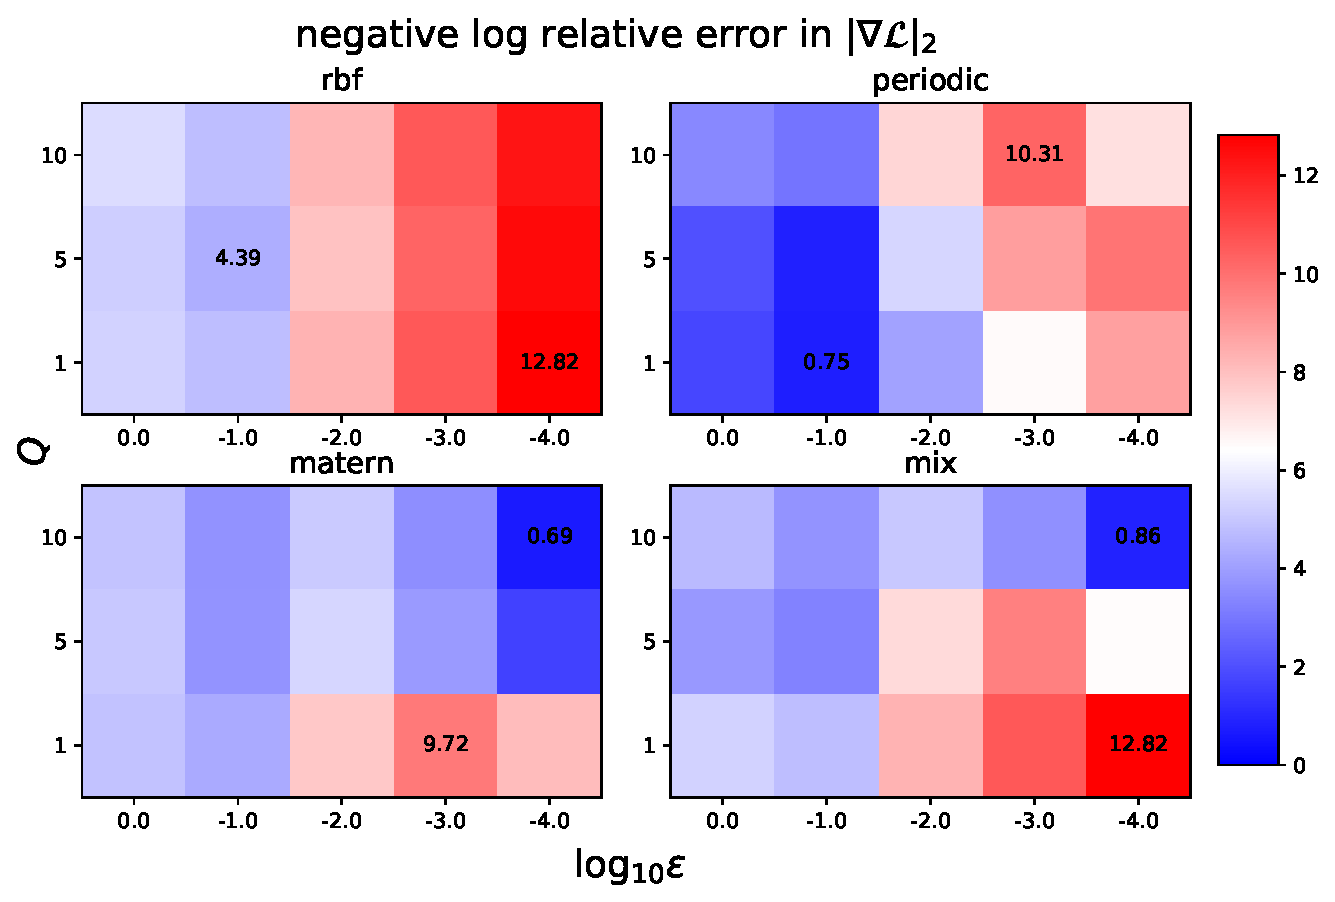
\includegraphics[width=\columnwidth]{relgrad_l2.eps}}
\caption{Negative logarithm of the relative error in $\ell_2$ norm between exact and LLGP gradients. Higher is better, and extremal values are noted.  For each data point, the average was taken over five runs.}
\label{fig:relgrad}
\end{center}
\vskip -0.1in
\end{figure}

\begin{figure}[!ht]
\vskip 0.1in
\begin{center}
\centerline{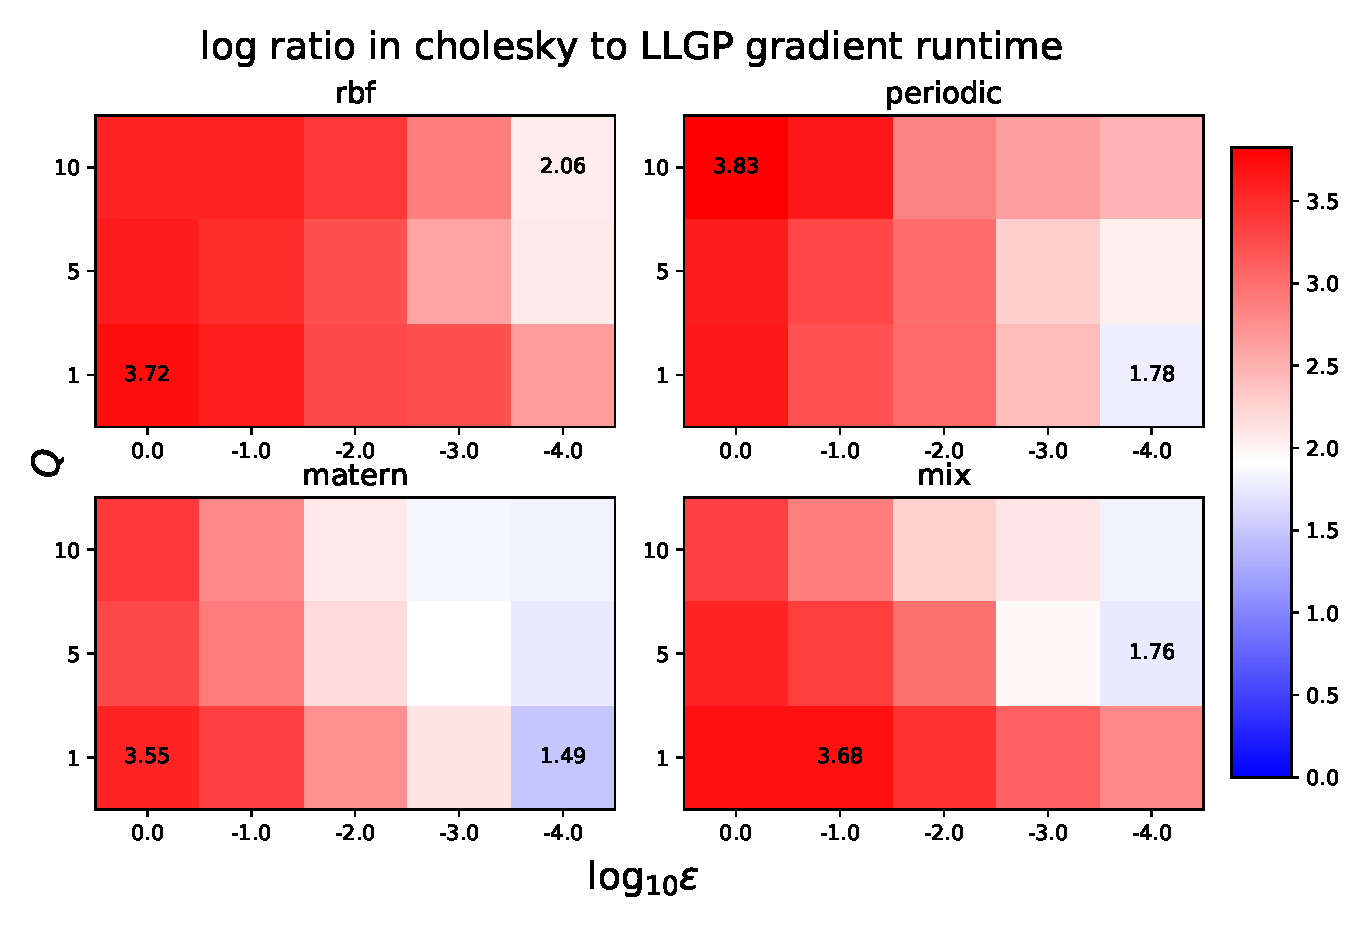
\includegraphics[width=\columnwidth]{time_ratio.eps}}
\caption{Logarithm of the ratio of time required by the exact approach to that of LLGP for computing the gradient over all parameters from Eq.~\ref{llgradient}. Higher is better, and extremal values are noted. For each data point, the average was taken over five runs.}
\label{fig:gradtime}
\end{center}
\vskip -0.1in
\end{figure}

\begin{figure}[!ht]
\vskip 0.1in
\begin{center}
\centerline{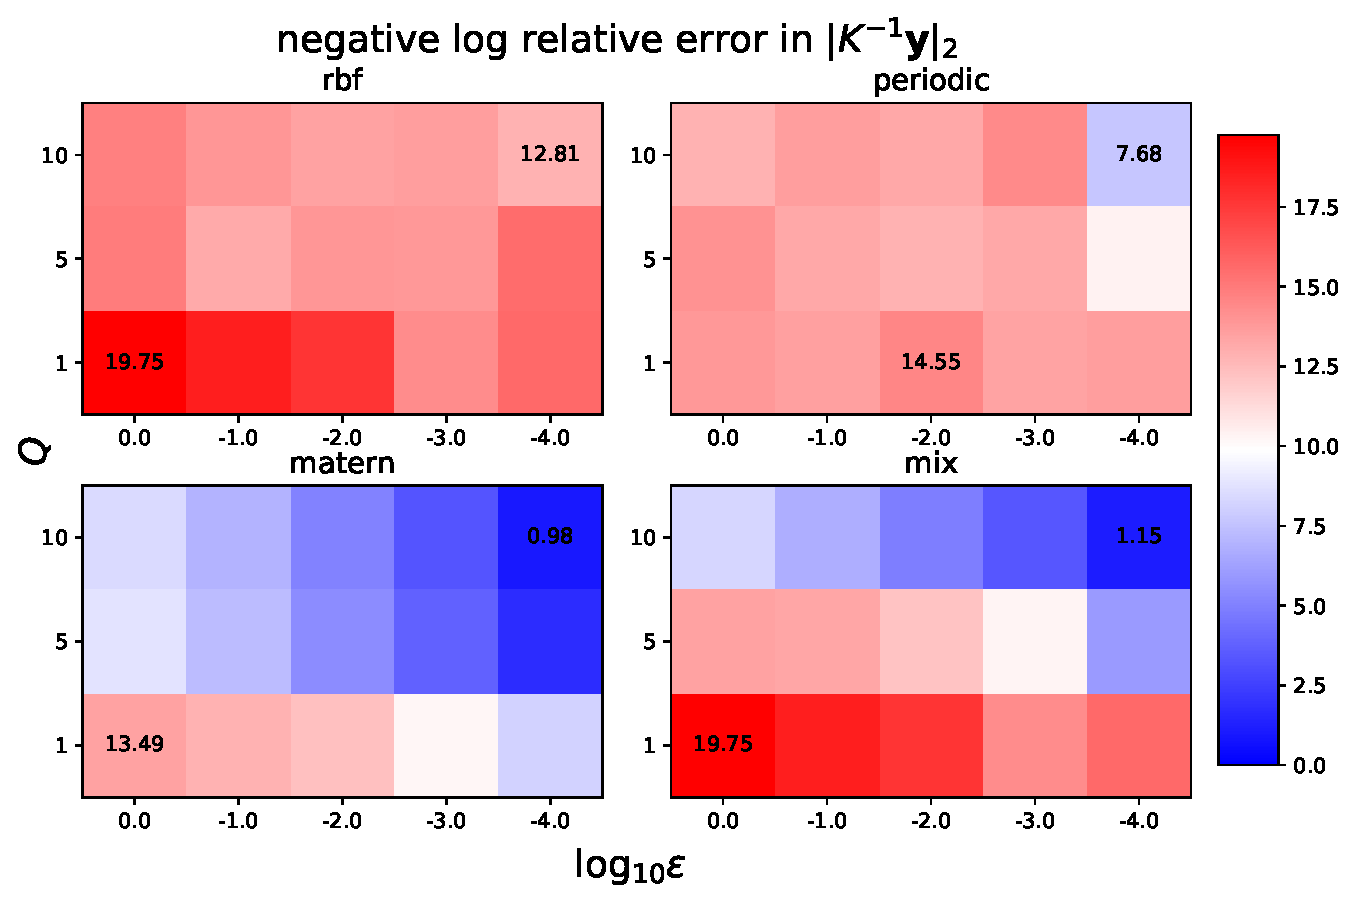
\includegraphics[width=\columnwidth]{relalpha_l2.eps}}
\caption{Negative logarithm of the relative error in $\ell_2$ norm between exact and MINRES solutions to $K\Tx=\Ty$ for $\Tx$. For each data point, the average was taken over five runs.}
\label{fig:inverr}
\end{center}
\vskip -0.1in
\end{figure}

\subsection{Foreign exchange rate prediction (FX2007)}\label{fx2007-results}

We replicate the medium-sized dataset from COGP as an application to evaluate LLGP performance. The dataset consists of ten foreign currency exchange rates---CAD, EUR, JPY, GBP, CHF, AUD, HKD, NZD, KRW, and MXN---and three precious metals---XAU, XAG, and XPT---implying that $D=13$.\footnote{Data are from \url{http://fx.sauder.ubc.ca/data.html}} As in COGP, we retrieved the asset to USD rate, then used its reciprocal in all the results discussed below. The LLGP setting has $Q=1,R=2$, as recommended in \cite{alvarez2010efficient} for LMC models on this dataset; let this be the LMC model on LLGP. COGP roughly corresponds to the the SLFM model, which has a total of 94 hyperparameters, compared to 53 for LLGP. All kernels are RBF.

The data used in this example are from 2007, and include $n=3054$ training points and $150$ test points. The test points include 50 contiguous points extracted from each of the CAD, JPY, and AUD exchanges.

For this application, LLGP uses $m=n/D=238$ interpolating points. We use the COGP settings from the paper.\footnote{COGP hyperparameters for FX2007 were 100 inducing points, 500 iterations, 200 mini-batch size.} LLGP, for both LMC, outperforms COGP in terms of predictive mean and variance estimation as well as runtime (Tab.~\ref{fx2007-tbl}).

\begin{table}[!ht]
  \caption{Average predictive performance and training time over $10$ runs for LLGP and COGP on the FX2007 dataset. Parenthesized values are standard error. LLGP was run with LMC set to $Q=1$, $R=2$, and $238$ interpolating points. COGP used a $Q=2$ kernel with $100$ inducing points.}
\label{fx2007-tbl}
\vskip 0.15in
\begin{center}
  \begin{small}
    \begin{sc}
      \begin{tabular}{|l|cc|}\hline\abovespace\belowspace
Metric & LLGP & COGP\\
\hline\abovespace
seconds & $\textbf{100}$ ($\textbf{13}$) & $731$ ($194$)\\
SMSE & $\textbf{0.21}$ ($\textbf{0.01}$) & $0.26$ ($0.03$)\\
NLPD & $\textbf{-3.62}$ ($\textbf{0.07}$) & $14.52$ ($3.10$)
\belowspace \\
\hline
\end{tabular}

\end{sc}
\end{small}
\end{center}
\vskip -0.1in
\end{table}

\begin{figure*}[!ht]
\vskip 0.1in
\begin{center}
\centerline{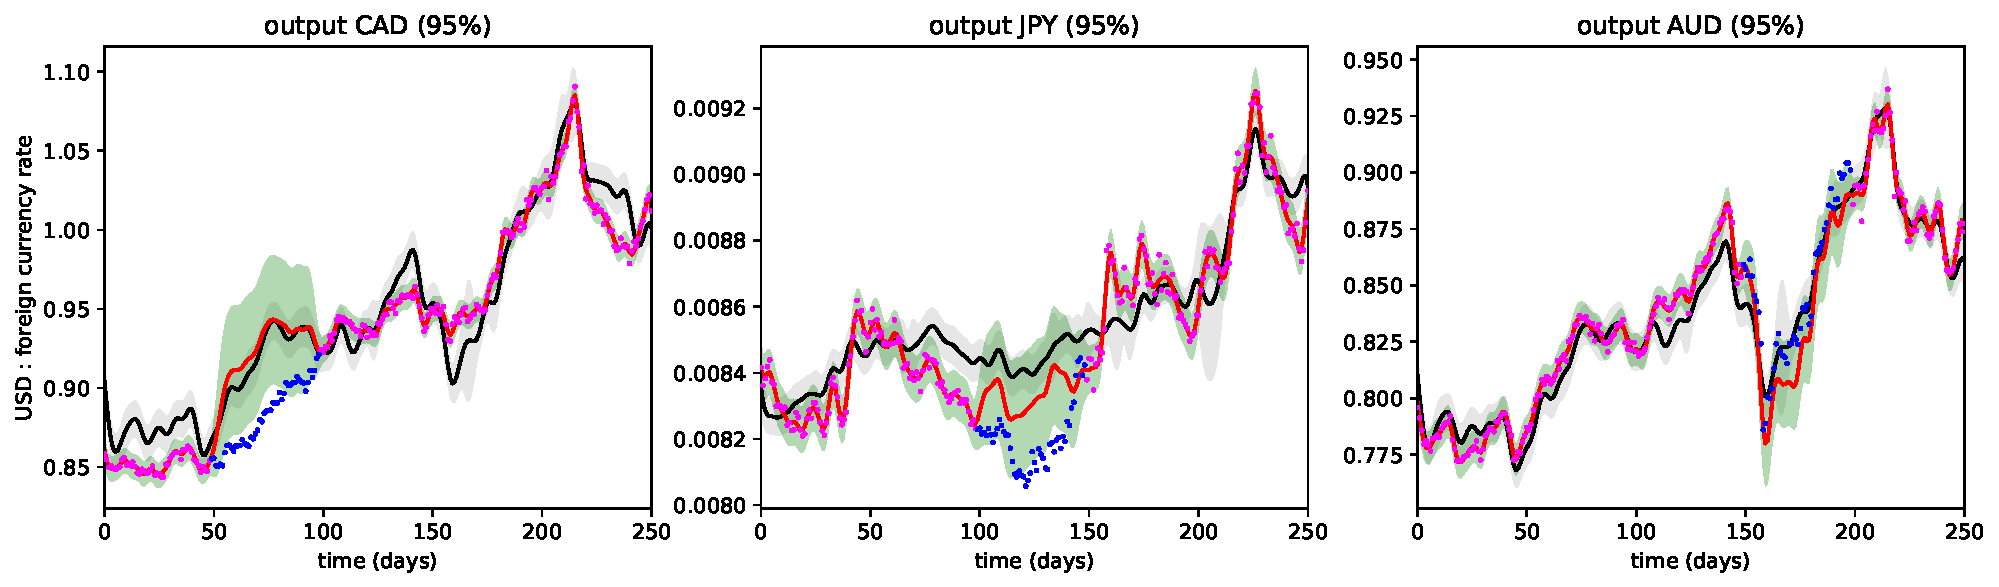
\includegraphics[width=\textwidth]{fx2007graph.pdf}}
\caption{Test outputs for the FX2007 dataset. COGP mean is black, with 95\% confidence intervals shaded in grey. LLGP mean is a solid red curve, with light green 95\% confidence intervals. Magenta points are in the training set, while blue ones are in the test set. Notice LLGP variance corresponds to an appropriate level of uncertainty on the test set and certainty on the training set, as opposed to the uniform variance from COGP.}
\label{fx2007-graph}
\end{center}
\vskip -0.1in
\end{figure*}

\subsection{Weather dataset}\label{large-bench}

Next, we replicate results from a weather dataset, a large time series used to validate COGP. In this dataset, $D=4$ weather sensors Bramblemet, Sotonmet, Cambermet, and Chimet record air temperature over five days in five minute intervals, with some dropped records due to equipment failure. Parts of Cambernet and Chimet are dropped for imputation, yielding $n=15789$ training measurements and $374$ test measurements. 

We use the COGP parameters that were set by default in the code provided by the authors.\footnote{\url{https://github.com/trungngv/cogp}, commit \texttt{3b07f621ff11838e89700cfb58d26ca39b119a35}. The weather dataset was run on 1500 iterations, mini-batch size 1000.} LLGP was run with the same parameters as in FX2007, simulating the SLFM model. We tested LLGP models on different numbers of interpolating points $m$.

\begin{table}[!ht]
  \caption{Average predictive performance and training time over $10$ runs for LLGP and COGP on the weather dataset. Parenthesized values are standard error. Both LLGP and COGP trained the SLFM model. We show LLGP with $500$ and $1000$ interpolating points and COGP with $200$ inducing points.}
\label{weather-tbl}
\vskip 0.15in
\begin{center}
  \begin{small}
    \begin{sc}
      \begin{tabular}{lccc}\toprule
Metric & \begin{tabular}{c}LLGP\\$m=500$\end{tabular} & \begin{tabular}{c}LLGP\\$m=1000$\end{tabular} & COGP\\
\midrule
seconds & $\textbf{126}$ ($\textbf{33}$) & $582$ ($154$) & $1214$ ($10$)\\
SMSE & $0.09$ ($0.01$) & $0.09$ ($0.01$) & $\textbf{0.08}$ ($\textbf{0.00}$)\\
NLPD & $2.14$ ($0.58$) & $\textbf{1.54}$ ($\textbf{0.03}$) & $98.55$ ($1.27$)\\

\bottomrule
\end{tabular}

\end{sc}
\end{small}
\end{center}
\vskip -0.1in
\end{table}

LLGP performed slightly worse than COGP in SMSE, but both NLPD and runtime indicate significant improvements (Tbl.~\ref{weather-tbl}). Varying the number of interpolating points $m$ from $500$ to $1000$ constructs a tradeoff frontier between increases in $m$ and NLPD decrease at the cost of additional runtime (Fig.~\ref{fig:llgpweather}). While NLPD improvement diminishes as $m$ increases, LLGP is still an improvement compared to COGP for a range of $m$ by an order of magnitude in runtime and almost two orders of magnitude for NLPD.

\begin{figure}[!ht]
\vskip 0.1in
\begin{center}
\centerline{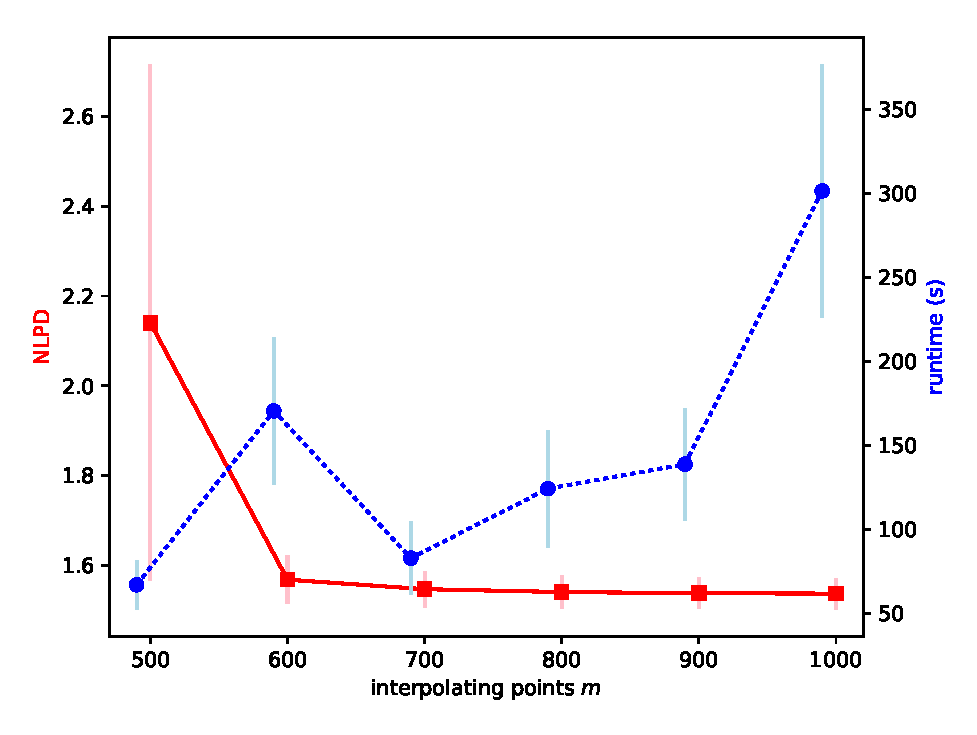
\includegraphics[width=\columnwidth]{m_time_nlpd.eps}}
\caption{Average and standard error of NLPD and runtime of the SLFM model on LLGP across over varying interpolating points. Every setting was run 10 times.}
\label{fig:llgpweather}
\end{center}
\vskip -0.1in
\end{figure}
\section{Conclusion}\label{conclusion}

LLGP recovers speedups from SKI \cite{kiss-gp} for the problem of multi-output GP regression by recognizing structure unique to LMC kernels, and otherwise not necessarily recoverable in general multi-output kernels. This structure further enables a parsimonious representation that allows even large GPs to be learned without explicit construction of the covariance matrix.

LLGP provides a means to approximate the log-likelihood function gradients through interpolation. We have shown on several datasets that this can be done in a way that is faster and leads to more accurate results than variational approximations.

Future work would extend the inputs to accept multiple dimensions. This can be done without losing internal structure in the kernel \cite{msgp}: Toeplitz covariance matrices become block-Toeplitz with Toeplitz-blocks (BTTB). The cubic interpolation requires and exponential number of terms, so projection into lower dimensions learned in a supervised manner would be essential. Another useful line for investigation would be more informed stopping heuristics. Finally, an extension to non-Gaussian noise is also feasible in a matrix-free manner by following prior work \cite{cutajar2016preconditioning}.

\bibliography{paper}
\bibliographystyle{icml2017}

\end{document} 


%  LocalWords:  Feinberg pu Cheng Engelhardt Kai LLGP Bonilla COGP qA
%  LocalWords:  hyperparameter's nguyen Semiparametric SLFM Scalable
%  LocalWords:  MSGP vectorization matricization parameterization PSD
